\documentclass[a4paper, 14pt]{extarticle}

% Поля
%----------------------
\usepackage{geometry}
\geometry{a4paper,left=2cm,right=1cm,
    top=2cm,bottom=2cm,bindingoffset=0cm}
%----------------------

% Russian-specific packages
%----------------------
\usepackage[T2A]{fontenc}
\usepackage[utf8]{inputenc}
\usepackage[english, main=russian]{babel}
%----------------------

\usepackage{textcomp}

% Красная строка
%----------------------
\usepackage{indentfirst}
%----------------------

% Graphics
%----------------------
\usepackage{graphicx}
\graphicspath{ {./images} }
\usepackage{wrapfig}
%----------------------

% Import minted
%----------------------
\usepackage{minted}
%----------------------

\linespread{1.3}
\sloppy
\clubpenalty=10000
\widowpenalty=10000

\begin{document}

%--------------------------------------
%			ТИТУЛЬНЫЙ ЛИСТ
%--------------------------------------
\begin{titlepage}
\thispagestyle{empty}
\newpage


%Шапка титульного листа
%--------------------------------------
\vspace*{-60pt}
\hspace{-65pt}
\begin{minipage}{0.3\textwidth}
\hspace*{-20pt}\centering

\includegraphics[width=\textwidth]{emblem}
\end{minipage}
\begin{minipage}{0.67\textwidth}\small \textbf{
\vspace*{-0.7ex}
\hspace*{-6pt}\centerline{Министерство науки и высшего образования Российской Федерации}
\vspace*{-0.7ex}
\centerline{Федеральное государственное бюджетное образовательное учреждение }
\vspace*{-0.7ex}
\centerline{высшего образования}
\vspace*{-0.7ex}
\centerline{<<Московский государственный технический университет}
\vspace*{-0.7ex}
\centerline{имени Н.Э. Баумана}
\vspace*{-0.7ex}
\centerline{(национальный исследовательский университет)>>}
\vspace*{-0.7ex}
\centerline{(МГТУ им. Н.Э. Баумана)}}
\end{minipage}
%--------------------------------------

%Полосы
%--------------------------------------
\vspace{-25pt}
\hspace{-35pt}\rule{\textwidth}{2.3pt}

\vspace*{-20.3pt}
\hspace{-35pt}\rule{\textwidth}{0.4pt}
%--------------------------------------

\vspace{1.5ex}
\hspace{-35pt} \noindent \small ФАКУЛЬТЕТ\hspace{80pt} <<Информатика и системы управления>>

\vspace*{-16pt}
\hspace{47pt}\rule{0.83\textwidth}{0.4pt}

\vspace{0.5ex}
\hspace{-35pt} \noindent \small КАФЕДРА\hspace{50pt} <<Теоретическая информатика и компьютерные технологии>>

\vspace*{-16pt}
\hspace{30pt}\rule{0.866\textwidth}{0.4pt}
  
\vspace{11em}

\begin{center}
\Large {\bf Лабораторная работа № 4} \\ 
\large {\bf по курсу <<Языки и методы программирования>>} \\
\large <<Реализация итераторов в языке Java>> \\
\large Вариант 8
\end{center}\normalsize

\vspace{8em}


\begin{flushright}
  {Студент группы ИУ9-22Б Павлов И. П. \hspace*{15pt}\\ 
  \vspace{2ex}
  Преподаватель Посевин Д. П.\hspace*{15pt}}
\end{flushright}

\bigskip

\vfill
 

\begin{center}
\textsl{Москва 2023}
\end{center}
\end{titlepage}
%--------------------------------------
%		КОНЕЦ ТИТУЛЬНОГО ЛИСТА
%--------------------------------------

\newpage
\section{Цель работы}
Изучение обобщённых итераторов и экземплярных вложенных классов языка Java.

\section{Условие}
Во время выполнения лабораторной работы требуется разработать на языке Java один
из классов, перечисленных в таблицах 1 – 7. Класс должен реализовывать интерфейс Iterable.
Объект разрабатывемого класса должен быть изменяемым, то есть в нём надо так или
иначе предусмотреть возможность изменения внутреннего состояния.

Класс, представляющий множество дизъюнктов и частичное присваивание значений
переменным. Дизъюнкт – это формула, представляющая собой дизъюнкцию
булевских переменных.

Дизюнкт удобно представлять множеством имён переменных. Частичное
присваивание значений переменным может задаваться множеством имён
переменных, имеющих значение true. Итератор должен выдавать дизъюнкты,
принимающие значения true.

\section{Реализация основного класса}
{\scriptsize
\begin{minted}{java}
public class Main {
    public static void main(String[] args) {
        Disjunct myDisjunct1 = new Disjunct();
        Disjunct myDisjunct2 = new Disjunct();

        myDisjunct1.addVar("a", false);
        myDisjunct1.addVar("b", true);

        myDisjunct2.addVar("c", false);
        myDisjunct2.addVar("d", false);

        DisjunctSet mySet = new DisjunctSet();
        mySet.addDisjunct(myDisjunct1);
        mySet.addDisjunct(myDisjunct2);

        for (Disjunct ignored : mySet) {
            System.out.println("Элемент проверен.");
        }

        System.out.println("Значение первого дизъюнкта: " + myDisjunct1.isTrue());
        System.out.println("Значение второго дизъюнкта: " + myDisjunct2.isTrue());

        myDisjunct2.setVar("a", true);

        System.out.println("Второй дизъюнкт после изменения переменной: " + myDisjunct2.isTrue());
    }
}
\end{minted}
}

\section{Реализация Дизъюнкта}
{\scriptsize
\begin{minted}{java}
import java.util.HashSet;

public class Disjunct {
    private HashSet<String> trueVars = new HashSet<String>();
    private HashSet<String> vars = new HashSet<String>();

    public void addVar(String varName, boolean value) {
        if (value) {
            trueVars.add(varName);
        }
        vars.add(varName);
    }

    public void setVar(String varName, boolean value) {
        if (!value) {
            trueVars.remove(varName);
        } else {
            trueVars.add(varName);
        }
    }

    public boolean isTrue() {
        return trueVars.size() > 0;
    }

    @Override
    public String toString() {
        StringBuilder output = new StringBuilder("( ");
        for (String element : vars) {
            output.append(element).append(" ");
        }
        output.append(")");
        return output.toString();
    }
}

\end{minted}
}

\section{Реализация Множества Дизъюнктов}
{\scriptsize
\begin{minted}{java}
import java.util.HashSet;
import java.util.Iterator;

public class DisjunctSet implements Iterable<Disjunct> {
    public HashSet<Disjunct> disjuncts = new HashSet<Disjunct>();
    private int size;

    public DisjunctSet() {
        this.size = 0;
    }

    public void addDisjunct(Disjunct entity) {
        disjuncts.add(entity);
        this.size++;
    }

    @Override
    public Iterator<Disjunct> iterator() {
        return new setIterator();
    }

    private class setIterator implements Iterator<Disjunct> {

        private int currentIndex = 0;
        private final Iterator<Disjunct> internalIterator = disjuncts.iterator();

        @Override
        public boolean hasNext() {
            return this.currentIndex < size;
        }

        @Override
        public Disjunct next() {
            Disjunct nextDisjunct = internalIterator.next();
            currentIndex++;
            if (nextDisjunct.isTrue()) {
                System.out.println(nextDisjunct);
            }
            return nextDisjunct;
        }
    }
}
\end{minted}
}

\begin{figure}[h] 
\center{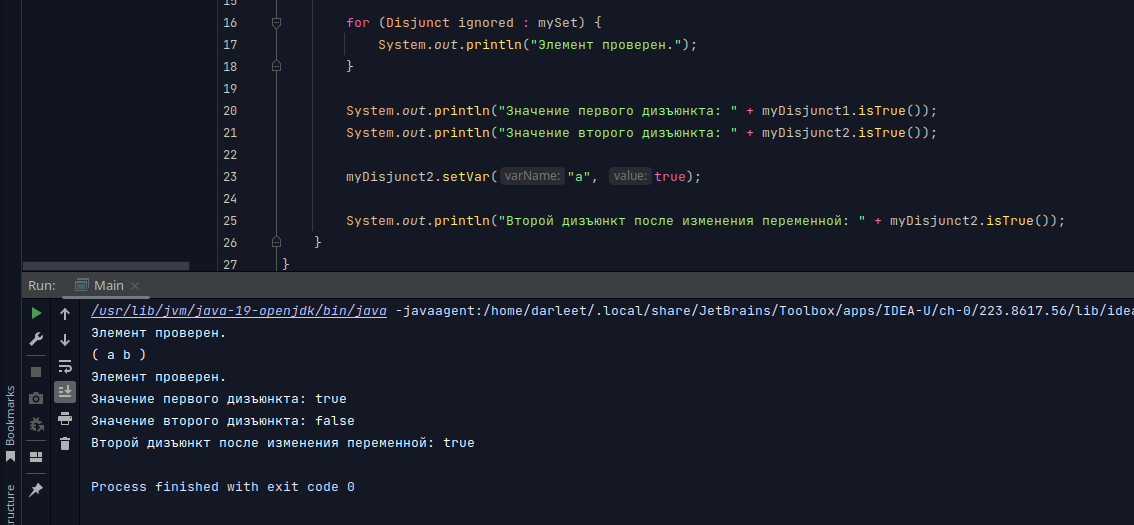
\includegraphics[scale=0.45]{class_main.png}} 
\caption{Вывод программы} 
\label{fig:image} 
\end{figure}

\end{document}
